\documentclass[11pt,oneside]{article}

\pdfminorversion=7
\usepackage{QuizStyle}
\usepackage{tikz}

\hypersetup{
    pdftitle={20261008 Quiz for MATH102 Calculus II},
    pdfauthor={Jungwoo Kim},
    pdfsubject={Quiz for MATH102 Calculus II},
    pdfcreator={LaTeX}
}

\begin{document}

\quiztitle{20261008 Quiz}

\begin{problem}{2.45}
Consider the polar coordinate mapping
\[
    \mathbf F(r,\theta)=(r\cos\theta,r\sin\theta),
    \qquad
    r\geq0,
    \quad
    0\leq\theta\leq2\pi.
\]
Sketch a region in the $(r,\theta)$-plane that corresponds to the upper half-plane $y>0$.
\end{problem}

\begin{solution}
Since $y=r\sin\theta$, the condition $y>0$ is equivalent, in the standard polar coordinate range, to
\[
    r>0,
    \qquad
    0<\theta<\pi.
\]
Thus the required region is
\[
    \boxed{\{(r,\theta)\in\R^2\mid r>0,\ 0<\theta<\pi\}}.
\]
A sketch in the $(r,\theta)$-plane is shown below.

\begin{center}
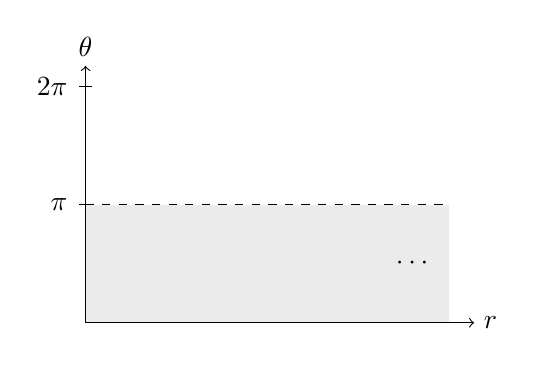
\begin{tikzpicture}[x=1.05cm,y=0.75cm]
    \fill[black!8] (0,0) rectangle (4.40,2.0);
    \draw[->] (0,0) -- (4.70,0) node[right] {$r$};
    \draw[->] (0,0) -- (0,4.35) node[above] {$\theta$};
    \draw[dashed] (0,2) -- (4.40,2);
    \draw (-0.08,2) -- (0.08,2);
    \draw (-0.08,4) -- (0.08,4);
    \node[left] at (-0.10,2) {$\pi$};
    \node[left] at (-0.10,4) {$2\pi$};
    \node at (3.95,1.00) {$\cdots$};
\end{tikzpicture}
\end{center}
\end{solution}

\begin{problem}{2.46}
Sketch the region in the $(x,y)$-plane that corresponds to the polar coordinate rectangle
\[
    1\leq r\leq2,
    \qquad
    0\leq\theta\leq\pi.
\]
Find the polar coordinates of the point $(x,y)=(0,1.5)$.
\end{problem}

\Needspace{22\baselineskip}
\begin{solution}
The condition $1\leq r\leq2$ places the points between the circles of radii $1$ and $2$, while $0\leq\theta\leq\pi$ restricts them to the upper half-plane.

Hence the image is
\[
    \boxed{\{(x,y)\in\R^2\mid y\geq0,\ 1\leq x^2+y^2\leq4\}},
\]
the closed upper half-annulus shown below.

\begin{center}
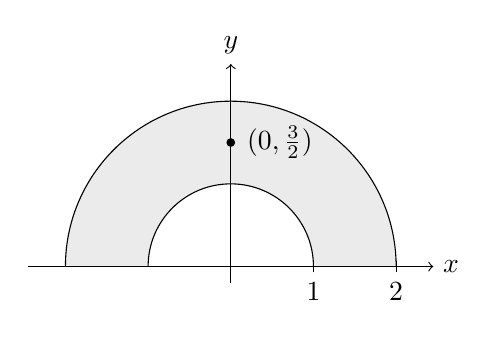
\begin{tikzpicture}[scale=1.05]
    \fill[black!8] (-2,0) arc[start angle=180,end angle=0,radius=2]
        -- (1,0) arc[start angle=0,end angle=180,radius=1] -- cycle;
    \draw[->] (-2.45,0) -- (2.45,0) node[right] {$x$};
    \draw[->] (0,-0.2) -- (0,2.45) node[above] {$y$};
    \draw (-2,0) arc[start angle=180,end angle=0,radius=2];
    \draw (-1,0) arc[start angle=180,end angle=0,radius=1];
    \draw (-2,0) -- (-1,0);
    \draw (1,0) -- (2,0);
    \draw (1,-0.07) -- (1,0.07);
    \draw (2,-0.07) -- (2,0.07);
    \node[below] at (1,-0.08) {$1$};
    \node[below] at (2,-0.08) {$2$};
    \fill (0,1.5) circle (1.5pt);
    \node[right] at (0.08,1.5) {$(0,\frac32)$};
\end{tikzpicture}
\end{center}

For $(x,y)=(0,1.5)$,
\[
    r=\sqrt{x^2+y^2}=\frac32,
    \qquad
    \theta=\frac\pi2.
\]
Therefore its polar coordinates are
\[
    \boxed{\left(r,\theta\right)=\left(\frac32,\frac\pi2\right)}.
\]
\end{solution}

\begin{problem}{2.47}
Use equations and inequalities to describe the following sets in polar coordinates.
\begin{problemsubparts}
    \item The open unit disk $x^2+y^2<1$.
    \item The first quadrant $x>0$, $y>0$.
\end{problemsubparts}
\end{problem}

\begin{solution}
Using $x^2+y^2=r^2$ and the standard ranges $r\geq0$ and $0\leq\theta\leq2\pi$,
\begin{problemsubparts}
    \item The open unit disk is described by
    \[
        \boxed{0\leq r<1,\qquad 0\leq\theta\leq2\pi}.
    \]

    \item In the first quadrant both $x=r\cos\theta$ and $y=r\sin\theta$ are positive. Thus
    \[
        \boxed{r>0,\qquad 0<\theta<\frac\pi2}.
    \]
\end{problemsubparts}
\end{solution}

\begin{problem}{2.49}
Let $0<b<a$ and consider the set of points in the plane whose polar coordinates $r,\theta$ satisfy
\[
    r=\frac{1}{a+b\cos\theta}.
\]
\begin{problemsubparts}
    \item Show that the $x,y$ coordinates of the points satisfy
    \[
        1=a\sqrt{x^2+y^2}+bx.
    \]
    \item Show that the equation
    \[
        1=a\sqrt{x^2+y^2}+bx
    \]
    is the equation of an ellipse by completing a square and getting the equation into the form
    \[
        1=\frac{(x-\alpha)^2}{c^2}+\frac{(y-\beta)^2}{d^2}.
    \]
\end{problemsubparts}
\end{problem}

\begin{solution}
\begin{problemsubparts}
    \item Multiplying the polar equation by $a+b\cos\theta$ gives
    \[
        1=ar+br\cos\theta.
    \]
    Since
    \[
        r=\sqrt{x^2+y^2},
        \qquad
        r\cos\theta=x,
    \]
    we obtain
    \[
        \boxed{1=a\sqrt{x^2+y^2}+bx}.
    \]

    \item From the equation in part (a),
    \[
        1-bx=a\sqrt{x^2+y^2}.
    \]
    Squaring and rearranging gives
    \[
        (a^2-b^2)x^2+2bx+a^2y^2=1.
    \]
    Since $0<b<a$, we have $a^2-b^2>0$. Completing the square in $x$ gives
    \[
        (a^2-b^2)
        \left(x+\frac{b}{a^2-b^2}\right)^2
        +a^2y^2
        =\frac{a^2}{a^2-b^2}.
    \]
    Therefore
    \[
        \boxed{
        1=
        \frac{\left(x+\dfrac{b}{a^2-b^2}\right)^2}
             {\dfrac{a^2}{(a^2-b^2)^2}}
        +
        \frac{y^2}{\dfrac{1}{a^2-b^2}}
        }.
    \]
    This is an ellipse with
    \[
        \alpha=-\frac{b}{a^2-b^2},
        \qquad
        \beta=0,
        \qquad
        c=\frac{a}{a^2-b^2},
        \qquad
        d=\frac{1}{\sqrt{a^2-b^2}}.
    \]
\end{problemsubparts}
\end{solution}

\begin{problem}{3.2}
Let
\[
    f(x,y)=x^2+3y.
\]
Find the linear approximation of $f(x,y)$ near $(2,4)$, and use it to estimate $f(2.01,4.03)$.
\end{problem}

\begin{solution}
We have
\[
    f(2,4)=16,
    \qquad
    f_x(x,y)=2x,
    \qquad
    f_y(x,y)=3.
\]
Thus
\[
    f_x(2,4)=4,
    \qquad
    f_y(2,4)=3,
\]
and the linear approximation at $(2,4)$ is
\[
    \boxed{L(x,y)=16+4(x-2)+3(y-4)}.
\]
Using this approximation,
\[
    f(2.01,4.03)
    \approx L(2.01,4.03)
    =16+4(0.01)+3(0.03)
    =16.13.
\]
Thus the requested estimate is
\[
    \boxed{f(2.01,4.03)\approx16.13}.
\]
\end{solution}

\begin{problem}{3.3}
Find the indicated partial derivatives of the functions.
\begin{problemsubparts}
    \item $f_x(x,y)$ and $f_y(2,0)$ if
    \[
        f(x,y)=e^{-x^2-y^2}.
    \]
    \item
    \[
        \frac{\partial}{\partial y}\left(xe^y+ye^x\right).
    \]
    \item
    \[
        \frac{\partial}{\partial x}
        \left(
            \cos(xy)+\frac{\partial}{\partial y}\sin(xy)
        \right).
    \]
\end{problemsubparts}
\end{problem}

\begin{solution}
\begin{problemsubparts}
    \item Differentiating with respect to $x$ gives
    \[
        \boxed{f_x(x,y)=-2xe^{-x^2-y^2}}.
    \]
    Also,
    \[
        f_y(x,y)=-2ye^{-x^2-y^2},
    \]
    so
    \[
        \boxed{f_y(2,0)=0}.
    \]

    \item Holding $x$ fixed,
    \[
        \boxed{
        \frac{\partial}{\partial y}\left(xe^y+ye^x\right)
        =xe^y+e^x
        }.
    \]

    \item First,
    \[
        \frac{\partial}{\partial y}\sin(xy)=x\cos(xy).
    \]
    Therefore
    \begin{align*}
        \frac{\partial}{\partial x}
        \left(
            \cos(xy)+\frac{\partial}{\partial y}\sin(xy)
        \right)
        &=\frac{\partial}{\partial x}\left(\cos(xy)+x\cos(xy)\right)\\
        &=\boxed{\cos(xy)-y\sin(xy)-xy\sin(xy)}.
    \end{align*}
\end{problemsubparts}
\end{solution}

\begin{problem}{3.6}
Consider the linear function
\[
    \ell(x,y,z)=ax+by+cz.
\]
Show that $\nabla\ell$ is constant. Show that when $a,b,c$ are not all zero, $\nabla\ell$ is normal to the level set $\ell=0$.
\end{problem}

\begin{solution}
The partial derivatives are
\[
    \ell_x=a,
    \qquad
    \ell_y=b,
    \qquad
    \ell_z=c,
\]
so
\[
    \boxed{\nabla\ell=(a,b,c)},
\]
which is constant.

Now let $\mathbf x=(x,y,z)$ lie in the level set $\ell=0$. Then
\[
    \nabla\ell\cdot\mathbf x
    =(a,b,c)\cdot(x,y,z)
    =ax+by+cz
    =0.
\]
Thus the level set $\ell=0$ is the plane through the origin orthogonal to $\nabla\ell$. Since $a,b,c$ are not all zero, $\nabla\ell\neq\mathbf 0$, so $\nabla\ell$ is a normal vector to the level set.
\end{solution}

\begin{problem}{3.11}
Define functions $f,g\colon\R^2\to\R$ by
\[
    f(x,y)=\cos(x+y),
    \qquad
    g(x,y)=\sin(2x-y).
\]
Find the gradients $\nabla f$ and $\nabla g$, and show that
\[
    f_x-f_y=0,
    \qquad
    g_x+2g_y=0.
\]
\end{problem}

\begin{solution}
For $f$,
\[
    f_x(x,y)=-\sin(x+y),
    \qquad
    f_y(x,y)=-\sin(x+y),
\]
so
\[
    \boxed{\nabla f(x,y)=\bigl(-\sin(x+y),-\sin(x+y)\bigr)}.
\]
Hence
\[
    f_x-f_y
    =-\sin(x+y)+\sin(x+y)
    =0.
\]

For $g$,
\[
    g_x(x,y)=2\cos(2x-y),
    \qquad
    g_y(x,y)=-\cos(2x-y),
\]
so
\[
    \boxed{\nabla g(x,y)=\bigl(2\cos(2x-y),-\cos(2x-y)\bigr)}.
\]
Hence
\[
    g_x+2g_y
    =2\cos(2x-y)-2\cos(2x-y)
    =0.
\]
\end{solution}

\end{document}
